%%%%%%%%%%%%%%%%%%%%%%%%%%%%%%%%%%%%%%%%%%%%%%%%%%%%%%%%%%%%%%%%%%%%%%
% How to use writeLaTeX:
%
% You edit the source code here on the left, and the preview on the
% right shows you the result within a few seconds.
%
% Bookmark this page and share the URL with your co-authors. They can
% edit at the same time!
%
% You can upload figures, bibliographies, custom classes and
% styles using the files menu.
%
%%%%%%%%%%%%%%%%%%%%%%%%%%%%%%%%%%%%%%%%%%%%%%%%%%%%%%%%%%%%%%%%%%%%%%

\documentclass[12pt]{article}
\usepackage{float}
\usepackage{booktabs}
\usepackage{tabulary}

\usepackage{caption}
\usepackage{subcaption}
\captionsetup{subrefformat=parens}
\usepackage{svg}
\usepackage{tikz}
\usepackage{pgfplots}
\usepackage{indentfirst} %alinhar 1 parágrafo

\usepackage{sbc-template}
\usepackage{graphicx}
\usepackage{dirtytalk}

\usepackage[T1]{fontenc}
\usepackage{mathtools}
\usepackage{blkarray, bigstrut}
\usepackage{gauss}
\usepackage{amsmath}
\usepackage{afterpage}
\usepackage{graphicx,url}
\usepackage{subcaption}
%\usepackage[brazil]{babel}
\usepackage[utf8]{inputenc}

\pgfplotsset{compat=1.10}
\usetikzlibrary{%
    intersections,%
    arrows,%
    decorations.pathmorphing,%
    backgrounds,%
    positioning,%
    fit,%
    petri,%
    calc,%
    through,%
    graphs,%
    shapes.misc,%
    trees,%
    mindmap,%
    shadows,%
    calendar%
}

\sloppy

\title{Machine learning methods in streamflow prediction  considering climate variable windowing}

\author{%
    Bruno T. R. V. Silva\inst{1}, %
    Carolina S. Ansélmo\inst{1}, \\%
    Paula C. S. Borba\inst{1}, %
    Wallace S. S. Souza\inst{1}%
}

\address{%
    Department of Civil Engineering -- Aeronautics Institute of Technology\\
    São José dos Campos, Brazil
    \email{bruno.valeriano@ga.ita.br, carolina.anselmo@ga.ita.br}%
    \vspace{-2ex}
    \email{paula.borba@ga.ita.br,  wallace.souza@ga.ita.br}
}

\begin{document}

\maketitle

\begin{abstract}
Hydropower operation and planning require streamflow forecasts. Machine learning methods combined with atmospheric climate variables complement physical models, particularly, where in-situ observations are not available. To make predictions of streamflow of a reservoir, we test four ML techniques: Support Vector Regressor (SVR), Simple Decision Tree, Random Forest (RF), and Stacking Regressor, which combines SVR, RF, and Ridge. Also, we add prediction horizon varying from 0 to 29 days for streamflow, and windowing of 1, 15, and 30 days for atmospheric climate variables. Results indicate a better fit in the RF model. Models outperform when a shorter horizon prediction of streamflow and longer windowing for climate variables are considered.

\end{abstract}


\section{Introduction}
\label{sec:Introduction}

Over 63\% of the whole electricity supply in Brazil came from hydropower in 2019. However, Brazil faces reduced availability of hydro resources in recent years \cite{onsseca}. Factors as changes in rainfall-runoff and temperature patterns affect the physical process of streamflow and water level in reservoirs. Impacts of climate variability on hydro resources have become a growing concern, since it may affect negatively the electricity supply in coming years, particularly in countries highly dependent on hydropower, like Brazil. Therefore, the ability to assess and make predictions about the streamflow of reservoirs allow important decisions to be made by competent authorities in order to ensure that water resources can be appropriately allocated.

Machine learning methods have been developed as a complement to physical hydrologic models, particularly, in contexts where data are limited to support those physical-based models. Further, the development of satellite data associated with in situ observations to monitor climate and hydrology makes available data of climate and streamflow more widely in data-poor regions \cite{julie}.

In this work, we make short-term forecast streamflow using Três Marias reservoir as study case. We use atmospheric variables as precipitation, evaporation, temperature, and surface runoff, available in Projeta project \cite{inpe}, and observed data of streamflow and water level of Três Marias reservoir \cite{onsnivel,onsvazao}. We compared four machine learning methods in order to access the best performance of short-term predictions. Moreover, we evaluate the impact of adding a horizon prediction of streamflow, as well as, windowing the climate variables.

In Section \ref{sec:RelatedBibliography}, the related bibliography regarding machine learning models in the context of streamflow prediction is introduced. The study area and data used for the modeling are presented in Section \ref{ssec:StudyAreaDecriptiveAnalysis}, while the pre-processing data and results are described in Section \ref{sec:DataPreprocessing}, followed by a analysis about the results in Section \ref{sec:ResultsDiscussion} and conclusion in Section \ref{sec:Conclusion}.

\section{Related bibliography}
\label{sec:RelatedBibliography}

Using physical or statistical models to study hydrological processes can raise several problems, such as high computational costs, weakness in uncertainty analysis and the need for a large number of comprehensive data \cite{ardabili2019deep}. Therefore, as a strategy to tackle some of these problems, machine learning methods, particularly Support Vector for Regression (SVR) and Random Forest (RF), have been growing in the water resource research community.

Support Vector for Regression (SVR) has an appropriate performance in solving small-scale, over-learning and nonlinear high-dimensional problems in the field of hydrological prediction \cite{xu,wang}. This regression model can be constructed using a nonlinear mapping function onto a high-dimensional space, in which the non-linear separable problem becomes linearly separable in space \cite{maity}. However, this model is highly dependent on kernel parameters.

Conventional decision tree learners generate a tree by splitting the data based on the values of predictors. Each node in the tree represents a test of some attribute, while each branch from that node is the possible value for that attribute.

Random Forest (RF) is also a widely used algorithm because of its satisfactory predictive power for time series \cite{wang}. Additionally, the model has the advantage of a simplified data pre-processing \cite{li}. The RF model combines a simple decision tree, in which each tree is generated by selecting random samples, and features from all predictors \cite{naghibi}.

According to \cite{dou}, ensemble machine learning techniques
provide an accurate and efficient solution in spatial modeling. Stacking ensemble ML algorithm learns how to combine the predictors from other well-performing models. In our case, we combined both SVR, RF models and Ridge regressors.

The natural complexity of hydrologic variables drives the approaches of mathematical models to actual output, in this case, streamflow. Although the selection of input variables varies according to the study, precipitation and temperature are common variables as observed in \cite{kassem2020predicting,essenfelder2020smart,bhatta2019evaluation}. Historical data of streamflow itself as input variable was present in \cite{li}. In order to approach the natural structure of a reservoir, we included in our work the variables runoff and evaporation, besides precipitation, evaporation, streamflow and water level.

\section{Material and methods}
\label{sec:MateriaMethods}

We selected Três Marias reservoir as a case study to forecast its short-term streamflow using four machine learning techniques: SVR, decision tree, RF and Stacking Regressor, combining SVR, RF and Ridge. We first describe the study area and data collection, then, we presented the parameters and applied methods of machine learning.

\subsection{Study area and descriptive analysis}
\label{ssec:StudyAreaDecriptiveAnalysis}

We chose Três Marias reservoir for two main reasons. First because of its importance to the Brazilian electricity system, since this reservoir holds a hydropower plant of 396 MW of installed capacity. Second, there are available atmospheric climate data at a high spatial resolution (5 km) for the Southeastern region, where Três Marias is located. Três Marias reservoir is inside the Alto São Francisco sub-basin in Minas Gerais state (Figure \ref{fig:studyarea}). We defined the river-group of each coordinate point using as reference \cite{fundep}.

\begin{figure}[htbp]
  \centering
  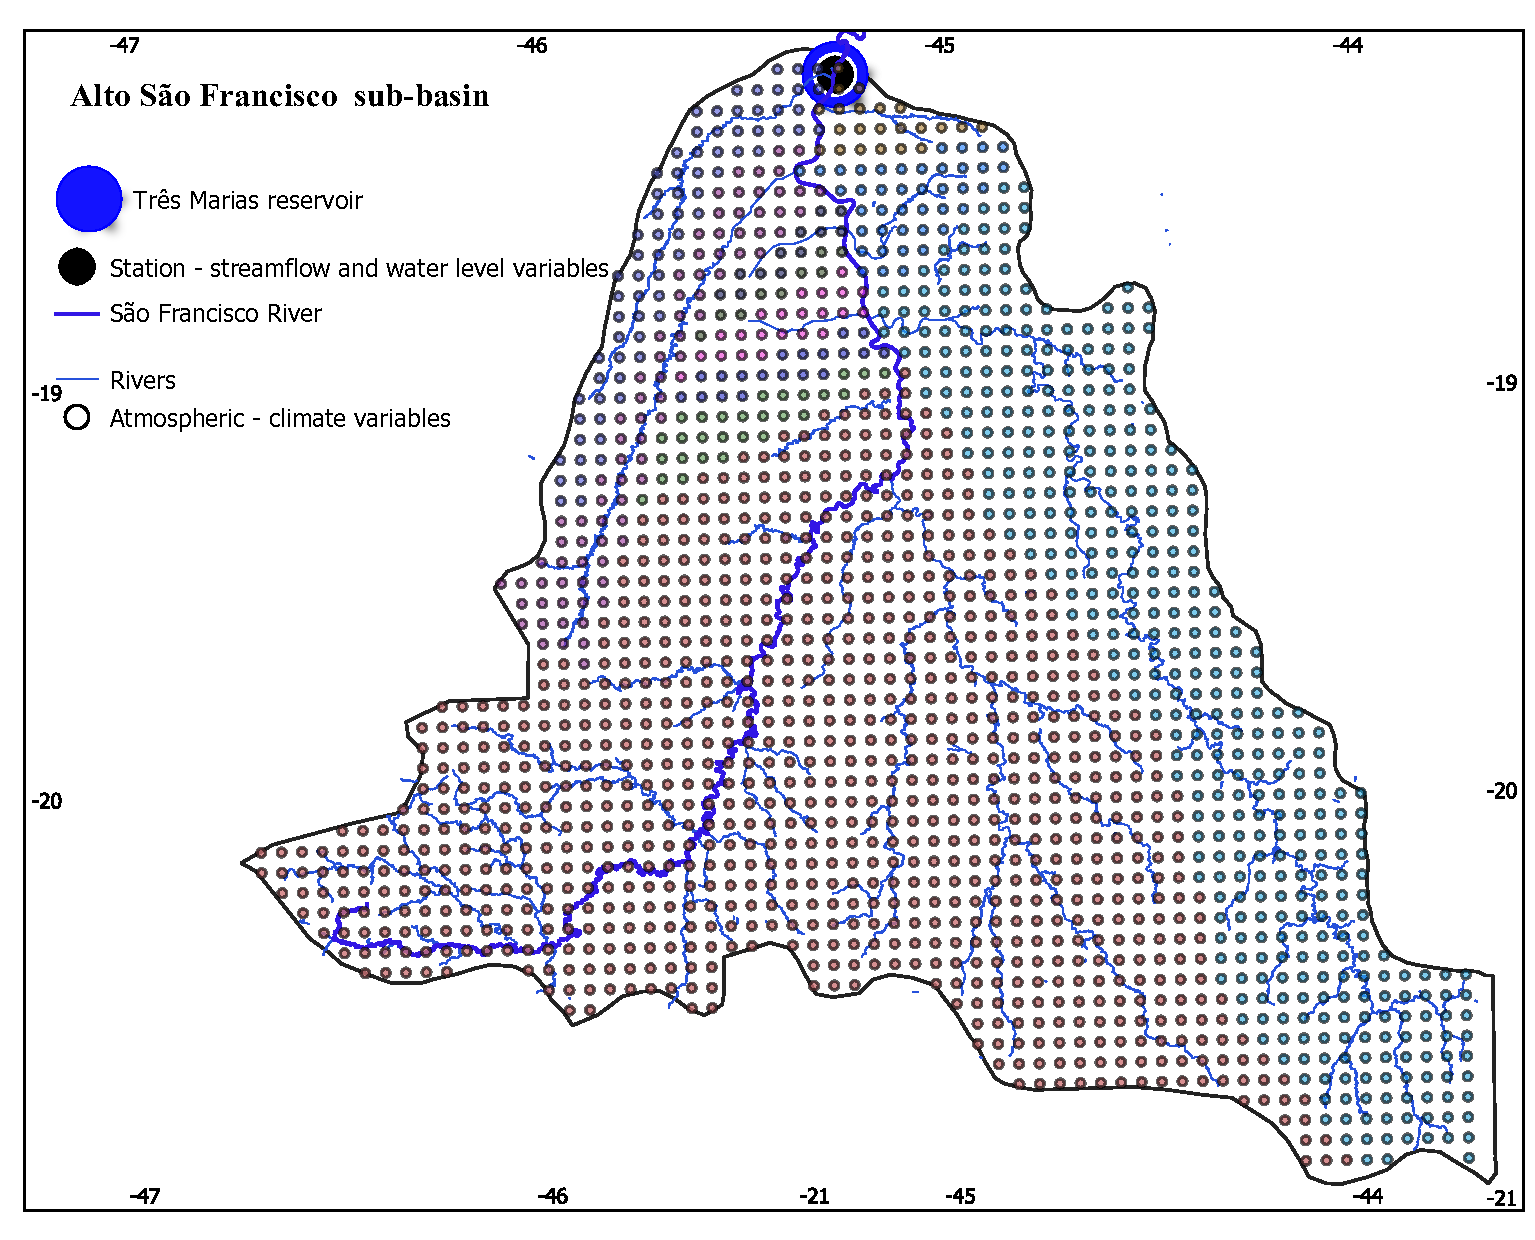
\includegraphics[width=0.9\linewidth]{Figures/mapa.pdf}
  \caption{Alto São Francisco sub-basin.}
  \label{fig:studyarea}
\end{figure}

\subsection{Data}
\label{ssec:Data}

We collected atmospheric climate data generated by CPTEC/INPE, available on the Projeta Platform \cite{chou2014assessment,chou2014evaluation,Lyra2018}, to forecast streamflow for Três Marias reservoir. The available data includes the period from January 1999 to December 2005. We combined that with observed data of streamflow and water level for the same period, available on \cite{onsnivel,onsvazao}. In our study, streamflow is the target variable, but its previous value is also input to the prediction. All variables are shown in Table~\ref{tab:predictors}. For further information of data exploration, see Appendix A.

\begin{table}[htbp]
\centering
\caption{Relation of predictors.}
\label{tab:predictors}
    %\resizebox{0.6\columnwidth}{!}{%
    \renewcommand{\arraystretch}{.8}
    \small\begin{tabulary}{\textwidth}{lcCcCr}
        \toprule
            \normalsize\bfseries{Variable} &
            \normalsize\bfseries{Unit} &
            \normalsize\bfseries{Temporal resolution} &
            \normalsize\bfseries{Historical data}  \\
        \midrule
            Temperature (T)    & ºC   & Daily   & 1999-2005 \\
            Precipitation (P)  & mm   & Daily   & 1999-2005 \\
            Evaporation (E)    & mm   & Daily   & 1999-2005 \\
            Surface runoff (R) & mm   & Daily   & 1999-2005 \\
            Streamflow (SF)    & m³/s & Daily   & 1999-2005 \\
            Water level (WL)   & m    & Daily   & 1999-2005 \\
            Month (M)          & -    & -       & 1999-2005 \\
        \bottomrule
    \end{tabulary}
    %}
\end{table}

%Descrever os dados: números de exemplos, de atributos, os tipos e escalas dos atributos, se é classificação/regressão, etc.. Se for classificação, dizer a proporção de exemplos na classe com mais observações (majoritária).

\subsection{Methods and evaluation criteria}
\label{ssec:MethodsEvaluation}

We tested four models: SVR, simple decision tree, RF and stacking ensemble method. We evaluated the performance of each model adding a windowing for climate variables in intervals of 1, 15, and 30 days. Furthermore, we tested horizon predictions varying from 0 to 29 days.

Using the python library Scikit-Learn \cite{scikit-learn}, we applied iterative steps, also known as pipelines, to detail the parameters and regression techniques. After these steps, we analyse the predictors results by the metrics R-squared score and Mean Absolute Error (MAE) to assess their performance. As shown in Figure \ref{fig:pipelines}, the developed pipeline starts by applying a time window transformation on precipitation, evaporation, temperature and surface runoff variables. This transformation consists in aggregating data from a specified time window, i.e., adding precipitation from the last fifteen or thirty days. Additionally, when evaluating SVR, data were normalized, as described in Section \ref{sec:DataTransformation}.

\begin{figure}[htbp]
    \centering
    {\footnotesize\includesvg[width=.8\linewidth]{Diagrams/gridsearch.drawio}}
    \caption{Pipeline setup for machine learning model search}
    \label{fig:pipelines}
\end{figure}

We used a combination of parameters to tune the model with an R-squared score as a metric, leveraging the GridSearchCV scikit-learn tool. In GridSearchCV, we define some constraints of each parameter, available in Appendix B. We adopted a cross-validation strategy to optimize these parameters and minimize the risk of overfitting. This was made to avoid testing regressor parameters on the same data it was trained for. The adopted approach was k-fold cross-validation, where the data set was divided into k groups - $k$ was set to 10 in this study - the regressors were trained in $k-1$ of these groups, and the fold left was used to test. As a consequence, the test was made using data the regressor have never seen while training. We calculate the final score as the average of the scores obtained for each test group.

To evaluate the performance of SVR, RF, Stacking Regressor and decision tree, we use two criteria: Mean Absolute Error (MAE) and R-squared. MAE represents the average of the absolute difference between the actual and predicted values. We included MAE as an error metric because it provides an interpretation of error on the same scale of streamflow. This procedure is represented by the Equation
    \begin{equation}
        \label{eqn:mae}
        MAE={\frac{1}{n}\sum_{i=0}^{n-1}|(X_{pred}-X_{i})|}
    \end{equation}
in which $n$ means the number of non-missing data, $i$ is the variable, $X_{pred}$ and $X_{i}$ mean the predicted and the actual value, respectively. Conversely, $R^2$ represents the proportion of the variance in the dependent variable which is explained by the regression model, and is given by the Equation
    \begin{equation}
        \label{eqn:r2}
        R^2={1 - \frac{\sum\limits_{i=0}^{n-1}(X_{pred}-X_{i})^{2}}
                      {\sum\limits_{i=0}^{n-1}(X_{i}-X_{mean})^{2}}}
    \end{equation}
where $X_{mean}$ is $\frac{1}{n}\sum_{i=0}^{n-1}X_{i}$, and $X_{pred}$ and $X_{i}$ are the predicted and it's corresponding true value, while $n$ is the size of the test sample. R-square is a indicator of goodness, indicating how well the model can predict unseen samples. The best possible R-squared value is $1.0$ and it can be negative, as the model gets arbitrarily worse.

\section{Data preprocessing}
\label{sec:DataPreprocessing}

We followed three main steps to organize the data into attribute-value format: data reduction, data integration, and data transformation. Other preprocessing procedures, such as feature selection, are not applicable since we filtered the data directly from Projeta Platform.

\subsection{Data reduction and integration}
\label{ssec:DataReductionIntegration}

Originally, we had a large dataset with the variables P, E, T, and R related to 1673 coordinate points inside the sub-basin limits in the period between 1999 to 2005.

We aggregated the coordinate points into 11 groups of rivers according to their contribution area to the Três Marias reservoir. We considered the daily sum for P and E, and the daily mean for T and R values. Thus, we created weather variables of P, E, T, and R for 11 groups of rivers instead of 1673 points. Additionally, we considered month as a qualitative attribute in order to capture seasonal changes in streamflow.

\subsection{Data transformation}
\label{sec:DataTransformation}

All variables, except month variable, were normalized when evaluating regressors that are sensitive to data scale, in order to prevent them from being dominated by variables with higher order of magnitude. We used the Min-Max normalization given by the Equation
    \begin{equation}
    \label{eqn:Normalization}
    x' = \frac{x-min(x)}{max(x)-min(x)}
    \end{equation}
to adjust the scale of the inputs. Where the value $x$ is the present value, $min(x)$ is the minimum value of the feature, and $max(x)$ is the maximum value of the feature. Then, we transformed that to their original scale.

While only the scale in the values changed with the normalization procedure, it is easier to identify the variation in mean and standard deviation between variables, as shown in Figure \ref{fig:Normalized} for the inputs in the first river.

\begin{figure}[htbp]
  \centering
  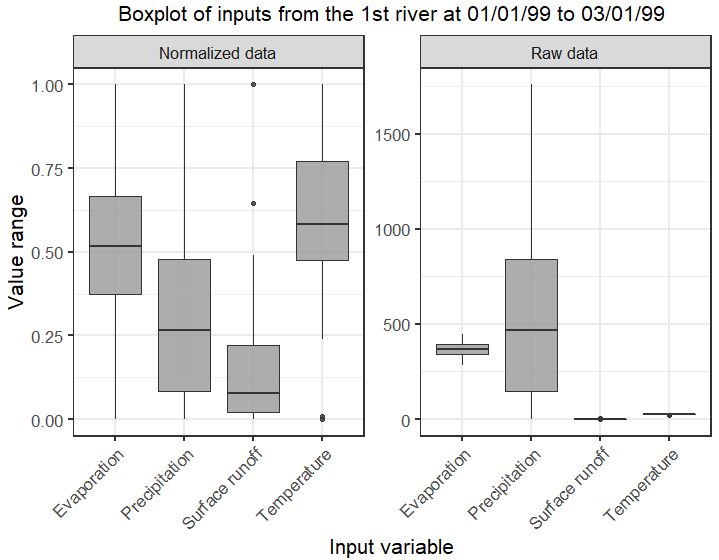
\includegraphics[width=0.8\linewidth, trim=0cm 0 0 .7cm,clip=true]{Figures/Normalização.png}
  \caption{Boxplot of inputs from normalized data (left) and raw data (rifht)}
  \label{fig:Normalized}
\end{figure}

For the month variable, we applied one-hot encoding, which is often used for categorical variables, when the regressor was sensitive to the scale of the attributes, such as SVR, or Ordinal encoding, otherwise.

\section{Results and discussion}
\label{sec:ResultsDiscussion}

Having tested horizon prediction of streamflow and water level varying from 1 to 29 days, and windowing at intervals of 1, 15 and 30 days for the climate variables, results indicated better fit for horizon of one day and window of 30 days. However, the models presented different results of R\textsuperscript{2} when they are compared to each other, as shown in Figure~\ref{fig:r2}.

\begin{figure}[htbp]
    \centering
    \begin{subfigure}[b]{.49\textwidth}
        \centering
        \includesvg{Graphs/R2_w01}
        \captionsetup{margin={.15\textwidth, 0cm}}
        \caption{1 day windowing}
        \label{fig:r2_1}
    \end{subfigure}
    \begin{subfigure}[b]{.49\textwidth}
        \centering
        \includesvg{Graphs/R2_w15}
        \captionsetup{margin={.15\textwidth, 0cm}}
        \caption{15 days windowing}
        \label{fig:r2_15}
    \end{subfigure}
    \begin{subfigure}[b]{\textwidth}
        \centering
        \includesvg{Graphs/R2_w30}
        \captionsetup{justification=justified,singlelinecheck=false}
        \captionsetup{margin={.23\linewidth, 0cm}}
        \caption{30 days windowing}
        \label{fig:r2_30}
    \end{subfigure}
    \caption{R\textsuperscript{2} for \subref{fig:r2_1} 1, \subref{fig:r2_15} 15, and \subref{fig:r2_30} 30 days windowing}
    \label{fig:r2}
\end{figure}

According to the increase of prediction horizon of streamflow up to 8 days, the R\textsuperscript{2} had an accentuated decrease in all models in 1 day-windowing. This trend is kept in 15 and 30 days windowing only for Decision Tree, while for SVR and Stacking Regressor the decrease is smaller and for Random Forest, R\textsuperscript{2} presented a growth.

Figure \ref{fig:sfigMAE} presents MAE values for different period-windowing and indicate how big of an error we can expect from the forecast on average. In all cases and models, the MAE values were greater than 100 m\textsuperscript{3}/s. However, MAE is higher for all models in 1 day-windowing case. In 15 and 30-days windowing, MAE was similar to each other, and greatly reduced if compared to 1 day-windowing. This suggests a better performance when climate data are analyzed within a greater windowing. In a physical process, that might represent the period of delay that climate variables, which were collected in the large sub-basin extension, have an impact on the upstream reservoir.

\begin{figure}[htbp]
    \centering
    \begin{subfigure}[b]{.49\textwidth}
        \centering
        \includesvg{Graphs/MAE_w01}
        \captionsetup{margin={.15\textwidth, 0cm}}
        \caption{1 day windowing}
        \label{fig:sfig1MAE}
    \end{subfigure}
    \begin{subfigure}[b]{.49\textwidth}
        \centering
        \includesvg{Graphs/MAE_w15}
        \captionsetup{margin={.15\textwidth, 0cm}}
        \caption{15 days windowing}
        \label{fig:sfig2MAE}
    \end{subfigure}
    \begin{subfigure}[b]{\textwidth}
        \centering
        \includesvg{Graphs/MAE_w30}
        \captionsetup{margin={.23\linewidth, 0cm}}
        \captionsetup{justification=justified,singlelinecheck=false}
        \caption{30 days windowing}
        \label{fig:sfig3MAE}
    \end{subfigure}
    \caption{Mean Absolute Errors (MAE) for \subref{fig:sfig1MAE} 1, \subref{fig:sfig2MAE} 15, and \subref{fig:sfig3MAE} 30 days windowing}
    \label{fig:sfigMAE}
\end{figure}

Analyzing the prediction horizon, results indicate that MAE tends to be constant for SVR and Decision Tree after 8 days of the horizon. MAE in RF model decreases slightly with the horizon time prediction expansion in 15 and 30 days-windowing.

From an evaluation of Figure~\ref{fig:StackedComparisson}, which demonstrates the true versus predicted values for 1 and 29 days of prediction horizon, it is evident that the model trained for 1 day of horizon presents greater sensitivity to sudden changes in reservoir streamflow, while that the model with the longest horizon time, despite being able to follow the streamflow trend, does not faithfully represent the peaks present. Another point that can be justified by the presence of these peaks is the relatively large value found for the MAE since the model ends up being highly penalized by sudden changes in streamflow. On the other hand, an R-squared metric, which considers the amplitude of the actual data, ends up not being penalized in the same way. Figure~\ref{fig:StackedComparisson} presents data for a two-year window from 2000 to 2002, so data can be more easily visualized. For a visualization for the whole data range, see Appendix~\ref{sec:TrueVersusPredicted}

\begin{figure}[htbp]
    \centering
    \includesvg{Graphs/StackedComparisson}
    \caption{Comparison between true and predicted values for a prediction     horizon of 1 and 29 days. Visualization for a 2 year window, from 2000 to 2002}
    \label{fig:StackedComparisson}
\end{figure}

After 8 days of prediction horizon, the R\textsuperscript{2} tends to be constant in 15 and 30 days-windowing cases. In 1 day-windowing case, the models presented an unexpected performance, since the models had a turning point in 15 days-horizon, in which the performance reached its lowest point and rose again.

Random forest outperforms in all considered cases of prediction horizon and windowing in terms of R\textsuperscript{2}. Decision Tree Regressor has the worst fit, while SVR and Stacking Regressor had similar results, although Stacking Regressor slightly presents higher values of R\textsuperscript{2}.

Results indicated that the variable shifted streamflow lost its strength with the horizon increasing, while the models become more dependent on other variables, as indicated in Figure \ref{fig:CategorizedImportance}. The importance of month variable increases in 1 day-windowing until prediction horizon of 22 days, then starts decreasing. In 15 days-windowing, month variable importance increases until 15 days, has a reduction in 22 days, and then grows again. In the case of 30 days-windowing, evaporation becomes the most relevant variable.

\begin{figure}[htbp]
    \centering
    \begin{subfigure}[b]{.49\textwidth}
        \centering
        \includesvg{Graphs/CategorizedImportance_w01}
        \captionsetup{margin={.17\textwidth, 0cm}}
        \caption{1 day windowing}
        \label{fig:CategorizedImportance01}
    \end{subfigure}
    \begin{subfigure}[b]{.49\textwidth}
        \centering
        \includesvg{Graphs/CategorizedImportance_w15}
        \captionsetup{margin={.17\textwidth, 0cm}}
        \caption{15 days windowing}
        \label{fig:CategorizedImportance02}
    \end{subfigure}
    \begin{subfigure}[b]{\textwidth}
        \centering
        \includesvg{Graphs/CategorizedImportance_w30}
        \captionsetup{margin={.26\linewidth, 0cm}}
        \captionsetup{justification=justified,singlelinecheck=false}
        \caption{30 days windowing}
        \label{fig:CategorizedImportance03}
    \end{subfigure}
    \caption{Variable importance for \subref{fig:CategorizedImportance01} 1, \subref{fig:CategorizedImportance02} 15, and \subref{fig:CategorizedImportance03} 30 days windowing}
    \label{fig:CategorizedImportance}
\end{figure}

In general terms, RF had a better results of MAE, if compared to other models. SVR presented the worst result, while both Stacking Regressor and Decision Tree had similar results.

\section{Conclusion}
\label{sec:Conclusion}

In this work, we tested four methods to forecast streamflow using Três Marias reservoir as a study case. Results indicated that RF had the best fit over the models.  For one-day prediction horizon for streamflow and water level , models presented R-squared values in the range 0.7 to 0.9, but that decreases according to the increase of  prediction horizon. With regards to windowing of climate variables, the best fits occur when considering a 30 days-windowing, which might be related to the delay of the physical process impact of all climate variables in the entire sub-basin on the reservoir upstream.

SVR had the highest values of MAE, while RF had the lowest values. The Stacking Regressor and decision tree produced similar values of MAE. Surprisingly, RF presented a slight increase of MAE for increased prediction horizon, and for the case of 15 and 30 days-windowing, while the other models presented a trend of having a decline.

Empirical results obtained from these models showed the performance not only over the models, but also changing the lag of streamflow and water level, and the window period of climate variables. That is important in solving water resources management problems and improve the streamflow prediction.

As the prediction horizon increases, the tested models become less sensitive to drastic changes in the streamflow, not being able to predict peaks, but keeping the ability to describe the overall tendency.

Finally, other properties that have a direct impact on streamflow, as land-use, soil classification, and wind speed, might improve the approach of modeling to the actual physical phenomena. Thus, we suggest the inclusion of other climate variables, and also other reservoir study cases.

\bibliographystyle{sbc}
\bibliography{sbc-template}

\appendix
\section{Data exploration}

  \begin{figure}[H]
  \centering
  \includesvg[width=.6\linewidth]{Figures/hist_prec.svg}
  \caption{Histogram of precipitation.}
  \end{figure}

    \begin{figure}[H]
  \centering
  \includesvg[width=.6\linewidth]{Figures/hist_temp.svg}
  \caption{Histogram of temperature.}
  \end{figure}

    \begin{figure}[H]
  \centering
  \includesvg[width=.6\linewidth]{Figures/hist_evap.svg}
  \caption{Histogram of evaporation.}
  \end{figure}

    \begin{figure}[H]
  \centering
  \includesvg[width=.6\linewidth]{Figures/hist_rnof.svg}
  \caption{Histogram of surface runoff.}
  \end{figure}

      \begin{figure}[H]
  \centering
  \includesvg[width=.6\linewidth]{Figures/hist_streamflow.svg}
  \caption{Histogram of streamflow.}
  \end{figure}

      \begin{figure}[H]
  \centering
  \includesvg[width=.6\linewidth]{Figures/hist_waterlevel.svg}
  \caption{Histogram of water level.}
  \end{figure}

\section{Parameters}
\noindent
\textbf{Support Vector Regression (SVR)}

\noindent
Kernel type: 'rbf' \\
Regularization parameter (c'): 15 to 31, step=5\\
Kernel coefficient for 'rbf' ($\gamma$)= scale/auto\\

\noindent
\textbf{Random Forest (RF)}

\noindent
The number of tree in the forest: 10, 100 or 250

\noindent
\textbf{Stacked regressor - SVR and RF}

\noindent
Combined parameters from SVR and RF.

\noindent
\textbf{Simple decision tree}

\noindent
Maximal decision tree: 5








\end{document}
